%background
\section{Parameters}
The ``input'' to a program is a set of parameters, named variables that represent specific data points. How those parameters are generated, and what literal form they take, affects the outcome of the program. Large programs with larger inputs may benefit from having their input parameter data sets generated by statistical distributions.

I was inspired to create this tool by testing a project I helped build in my software engineering class, which took in the records of each student in a class of 40 students, describing things like their skills in certain technologies and their available free times during the week. This project made a fairly sophisticated decision about how to form optimal groups of students to work in teams, ensuring that each group has complementary skills and overlapping free times. During testing, it is important to consider bizarre scenarios, like what should happen when no student has any free time at all, or when half the class can only meet early in the week and the other half can only meet late in the week.

These parameters can follow certain trends that can be mimicked by repeated trials of statistical distributions. The input to this program is merely an Excel csv file of a record table, such that every row is a student's entry and every column is all the entries for certain parameters that really effect the outcome of the program. Figure 2 shows the CSV file of the literal input into the Team Building program. The software takes in the filename, opens the file, and parses the data. Each row is a student, and each column is a parameter, such as free time availability on Monday or self-rated HTML experience level.

\begin{figure}
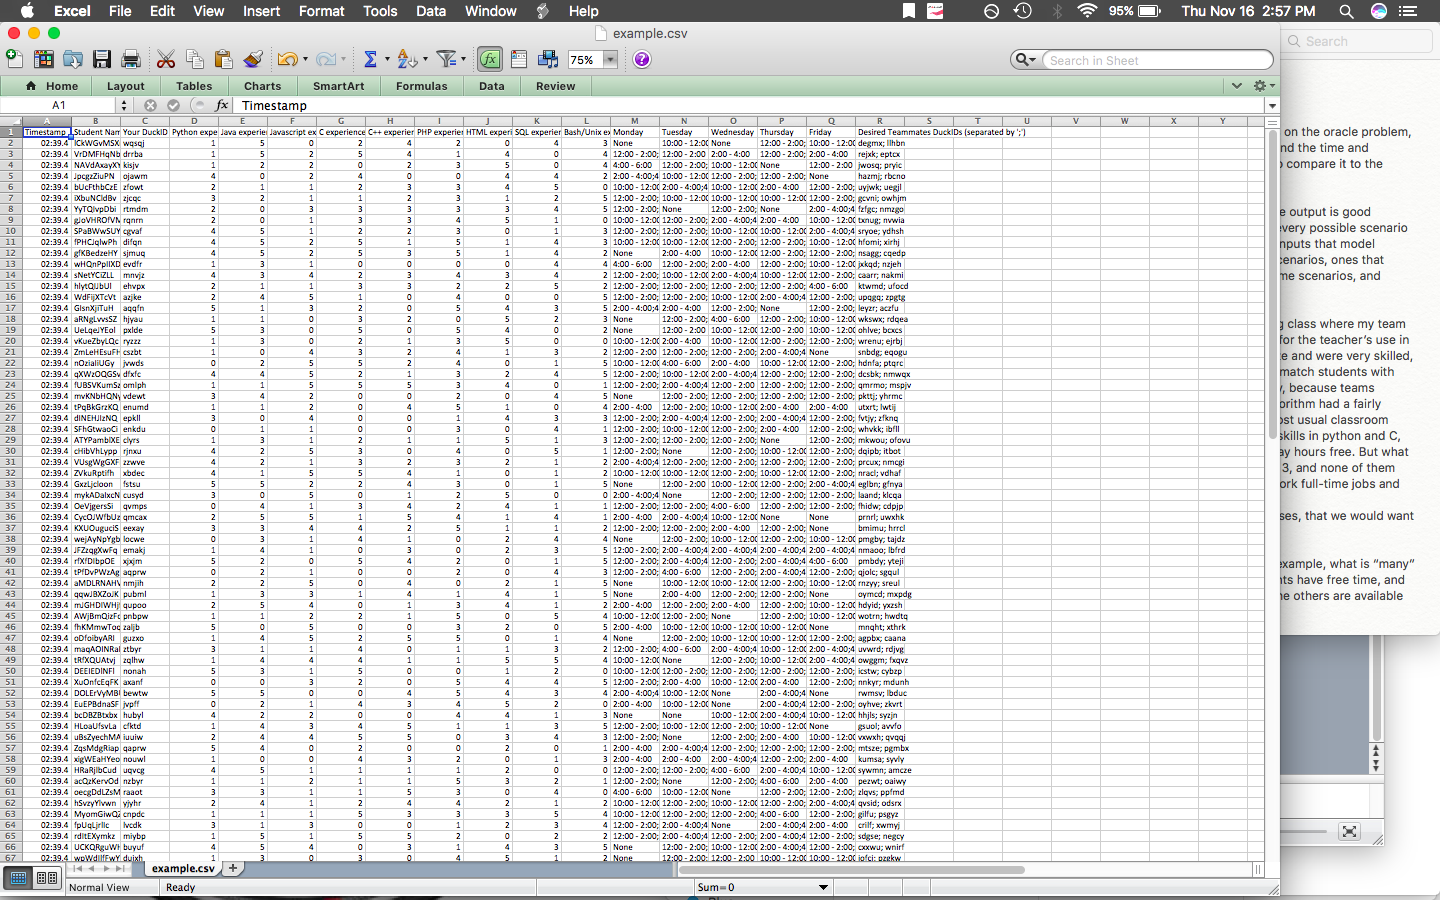
\includegraphics[]{team-file.png}
\end{figure}




\section{Pairwise Testing}
more stuf